\chapter{Studies of the inconsistency indexes for incomplete matrices}
\label{sec:studiesOfInconsistencyIndexesForIncompleteMatrices}

The presented inconsistency indexes were tested utilizing the Monte Carlo method. Their goal was to select those indexes which would give reliable results for incomplete matrices. Therefore, it was decided that the measure of the indexes' quality would be the \textit{relative error} (expressed as  percentage), which took into account the value of the index for a full, inconsistent matrix and the value of the index for the same matrix after partial decomposition. To be sure that the results were fair, all indexes were tested on the same set of matrices. The different sizes of the matrices, the levels of incompleteness and the levels of inconsistency were taken into account. Then, in order to compare the indexes easily and to select the best ones, the results were averaged using the arithmetic mean. The article \cite{Kazibudzki2017} was used while building the algorithm to solve the problem.


\section{Algorithm}
\subsection{Procedure steps:}
\begin{enumerate}
\item Randomly generate a vector $w=[w_{1},...,w_{n}]$ and a consistent PC matrix associated with it $PCM=\left(m_{ij}\right)$, where $m_{ij}=\frac{w_{i}}{w_{j}}$.
\item Disrupt the matrix by multiplying its elements (excluding the diagonal) by the value of $d$, randomly selected from the range $\left(\frac{1}{x},x\right)$.

\item Replace the values $m_{ij}$, where $i<j$ by the values $m_{ji}$.

\item Calculate the values of index with all the methods for the created matrix.

\item Remove some of the values from the matrix. The level of incompleteness should be $g$\%.

\item Calculate the values of inconsistencies by all methods for the incomplete matrix.

\item Calculate the relative error for each index.

\item Repeat steps 1 to 7 $X_{1}$ times.

\item Calculate the average relative error for each inconsistency index for the PC matrix.

\item Repeat steps 1 to 9 $X_{2}$ times.

\item Calculate the average relative error for each index by averaging the values obtained in step 9.

\end{enumerate}


\subsection{Details of the algorithm}
\label{sec:details}
The above algorithm was carried out for values $X_{1}=100$, $X_{2}=100$. Tests were started for values $d$ in range $\left(1.1,1.2,...,4\right)$ and then the results were averaged. It means that the average relative error of one index was calculated on the basis of 4000 matrices, each of which decomposed randomly 100 times. It gave together 400000 tests on how good the index was. 
\\
In addition, tests were carried out for various sizes of matrices.
\\
\\
\textbf{The results are divided into two parts:}
\begin{enumerate}
  \item A constant degree of incompleteness, different size of the matrix.
  \item Different degrees of incompleteness, constant size of the matrix.
\end{enumerate}

The aim of a such division is to pay attention to how the inconsistency indexes behave when the size of the matrix and the degree of incompleteness are changing. The results of the research are presented below.


\section{Implementation}

\subsection{Development environment}
Tests of indexes were developed in R language which is appropriate for numerical calculations (see \cite{projectR}). It contains sixteen of functions which support operations on matrices and vectors. Integrated development environment (IDE), named \textit{RStudio}, (see \cite{studioR}) was used during the implementation. This tool allows to create own packages which contain not only code but also documentation and information about licence and author. Using \textit{RStudio} package \texttt{indexesForIncomplete} was created. The most important part of this package is the file \texttt{indexes.R} which performs calculations necessary to test the indexes. \textit{RStudio} supports programmer's work by syntax highlighting, built-in console, easy documentation searching and many others. The program is available on common operating systems. Before using \textit{RStudio} one has to install \textit{R} programming language (see \cite{installR}).  



\begin{figure}[!]
\centerline{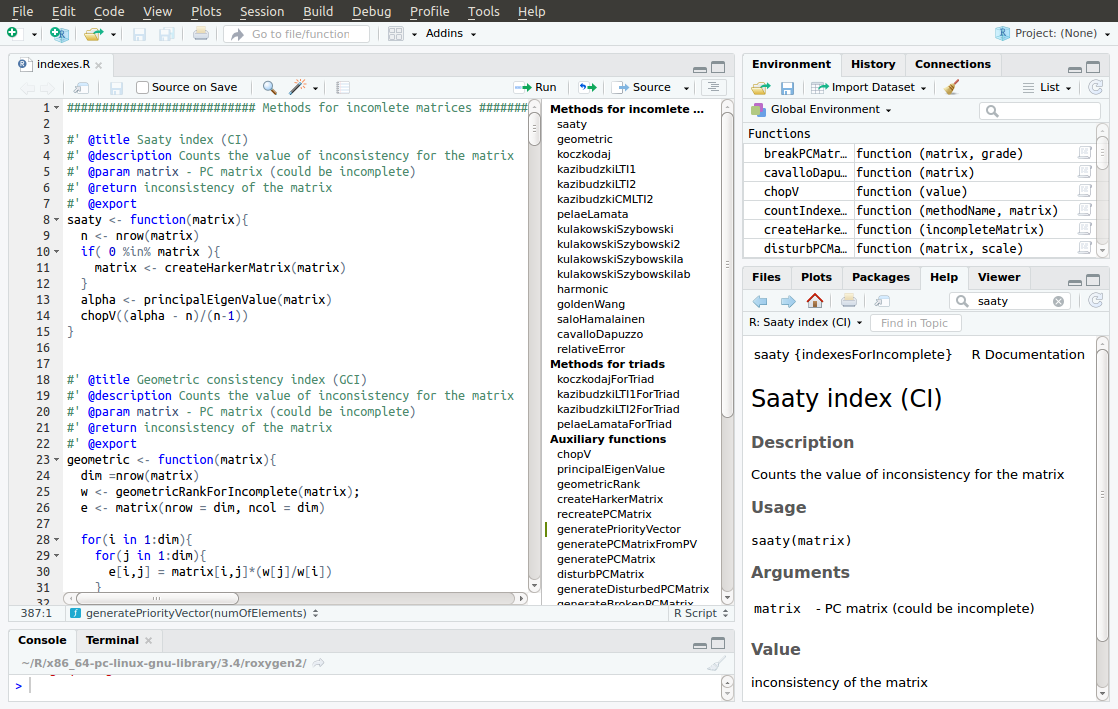
\includegraphics[width=\textwidth]{images/rstudio.png}}
\caption{Program \textit{RStudio}}
\label{fig:rstudio}
\end{figure}

\subsection{Implementation of the tests of the inconsistency indexes}
The implementation consists of two steps:
\begin{enumerate}
  \item Implementation of functions which calculate inconsistency indexes for a given matrix (full or incomplete).
  \item Implementation of functions which study indexes for different matrices and collect all the results of these tests. 
\end{enumerate}

\subsubsection{Implementation of the inconsistency indexes}
Sixteen functions which calculate the inconsistency indexes using methods are described in chapter 3. The functions were written in such a way that allows handling both full and incomplete matrices. The wrong matrices (it means nonreciprocal or inconsistent PC matrices) were not taken into account. Each of these function has only one parameter - \textit{PC matrix}. Exceptions are the two methods implementing Kulakowski and Szybowski index which additionally takes parameters $\alpha$ and $\beta$. The result of each function is a value of the inconsistency index. The functions were extended by comments which inform about the name of the index related to given function, parameters and returned value. It allows to read and modify the code easily. Several examples of the functions are presented below.

\begin{figure}[!]
\centerline{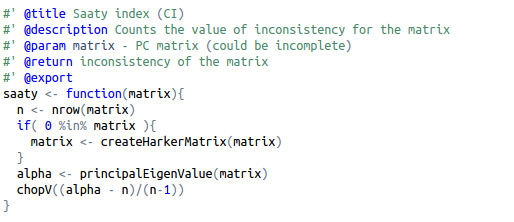
\includegraphics[scale=0.75]{images/kod1.png}}
\caption{The implementation of Saaty index}
\end{figure}

\begin{figure}[!]
\centerline{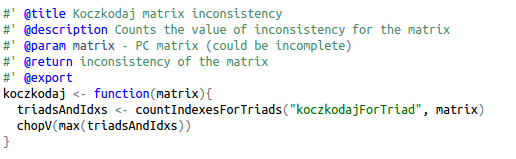
\includegraphics[scale=0.75]{images/kod2.png}}
\caption{The implementation of Koczkodaj index}
\end{figure}

\begin{figure}[!]
\centerline{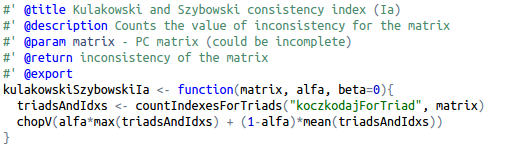
\includegraphics[scale=0.75]{images/kod3.png}}
\caption{The implementation of Kulakowski and Szybowski index ($I_{\alpha}$)}
\end{figure}

\begin{figure}[!]
\centerline{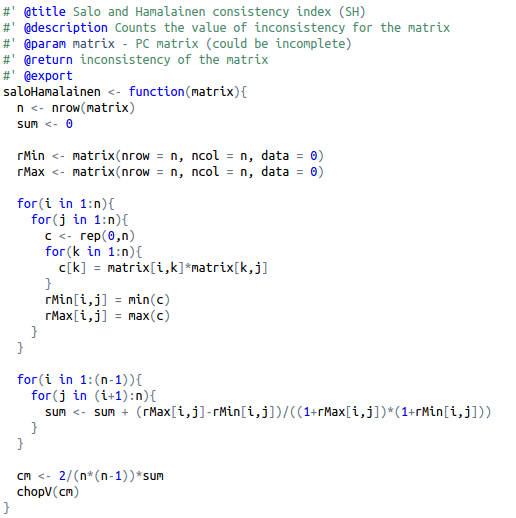
\includegraphics[scale=0.75]{images/kod4.png}}
\caption{The implementation of Salo and Hamalainen index}
\end{figure}
It is worth drawing attention to a function which is called within the functions intended for indexes based on triads. This function generates triads from a matrix and next returns inconsistency for each o them. The way to calculate inconsistency for one triad depends on a function passed as a parameter.

\begin{figure}[!]
\centerline{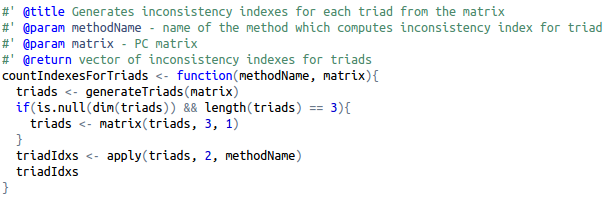
\includegraphics[scale=0.75]{images/kod5.png}}
\caption{The implementation of the function \texttt{countIndexesForTriads} which calculates inconsistency for each triad of a specified matrix}
\end{figure}

\newpage
\subsubsection{Implementation of tests}
In the second step, functions calculating the quality of the indexes for incomplete matrices, were created. Functions, which generate specified matrices, play an important role. PC matrices are created depending on the size, the level of inconsistency and the degree of incompleteness.

\begin{figure}[h]
\centerline{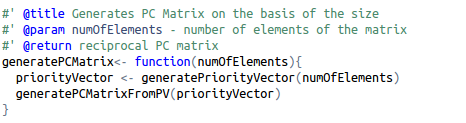
\includegraphics[scale=0.75]{images/kod11.png}}
\caption{The implementation of the function \texttt{generatePCMatrix} which generates the PC matrix depending on matrix size}
\end{figure}

\begin{figure}[h]
\centerline{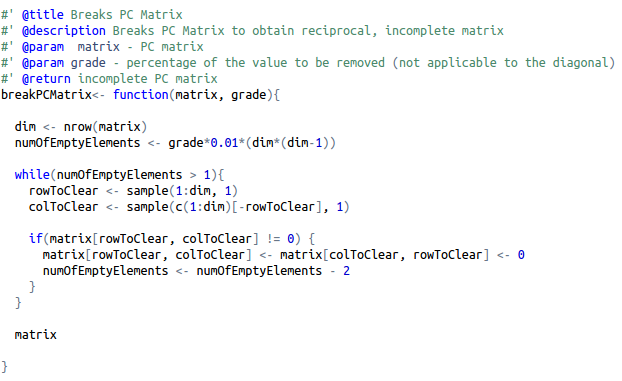
\includegraphics[scale=0.73]{images/kod13.png}}
\caption{The implementation of the function \texttt{breakPCMatrix} which breaks up the PC matrix regarding incompleteness depending on given degree of incompleteness}

\end{figure}


\begin{figure}[h]
\centerline{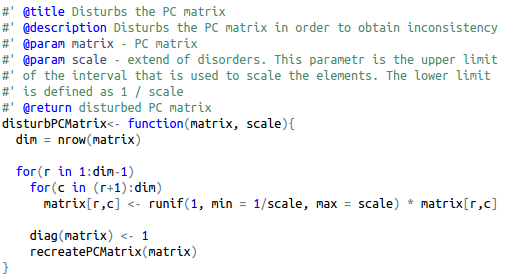
\includegraphics[scale=0.75]{images/kod12.png}}
\caption{The implementation of the function \texttt{disturbPCMatrix} which disturbs the PC matrix regarding inconsistency depending on given level of inconsistency}
\end{figure}


The last part of the functions relates to testing how big relative error occurs for inconsistency indexes after deleting some of the values. To begin with functions which test one index. They consider matrix size, the level of inconsistency, the degree of incompleteness and the number of attempts which are performed for a given matrix.

Then functions, which perform tests for each index, were implemented based on the same set of matrices. Thus, the results are reliable and each index is considered the same way.

\begin{figure}[h]
\centerline{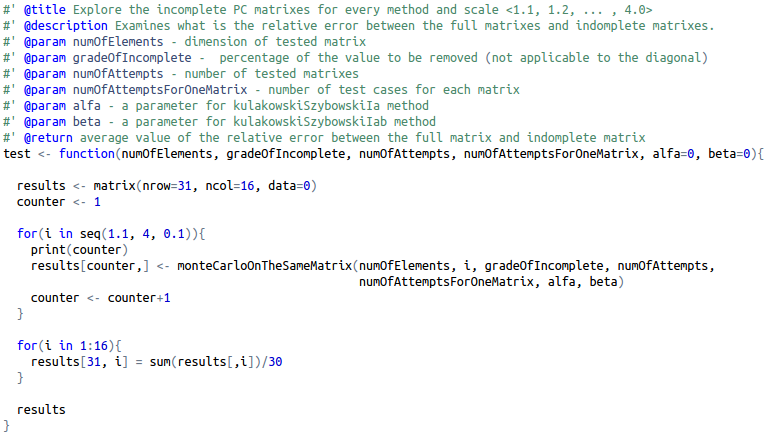
\includegraphics[scale=0.58]{images/kod22.png}}
\caption{The implementation of the function \texttt{test} which tests all indexes regarding given matrix size and the degree of incompleteness}
\end{figure}

\begin{figure}[h]
\centerline{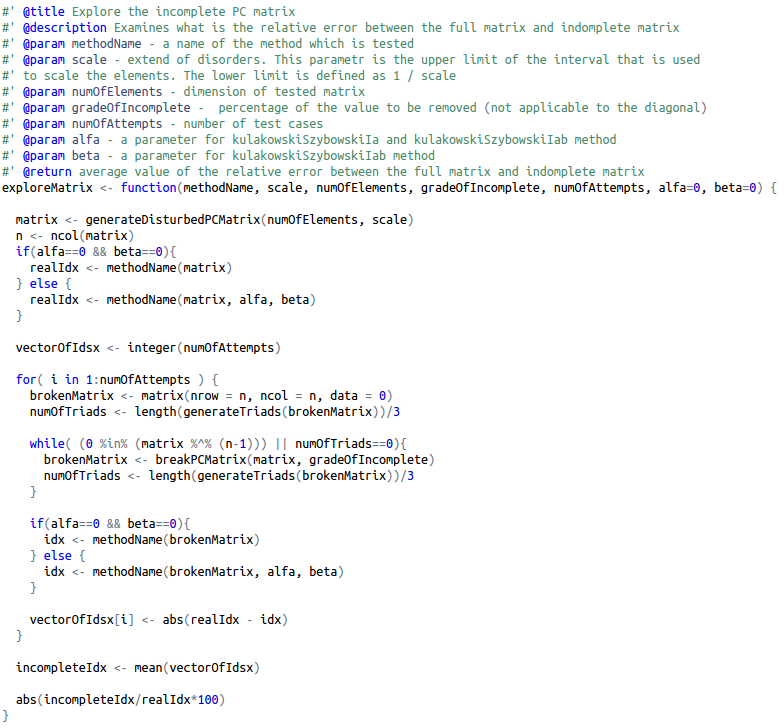
\includegraphics[scale=0.58]{images/kod21.png}}
\caption{The implementation of the function \texttt{exploreMatrix} which tests given inconsistency index}
\end{figure}



\clearpage
\subsection{Documentation}
Comments in code were used to generate the documentation. The package \texttt{roxygen2} were made for this purpose. \\ Exemplary portions of the documentation are presented below.

\begin{figure}[h]
\centerline{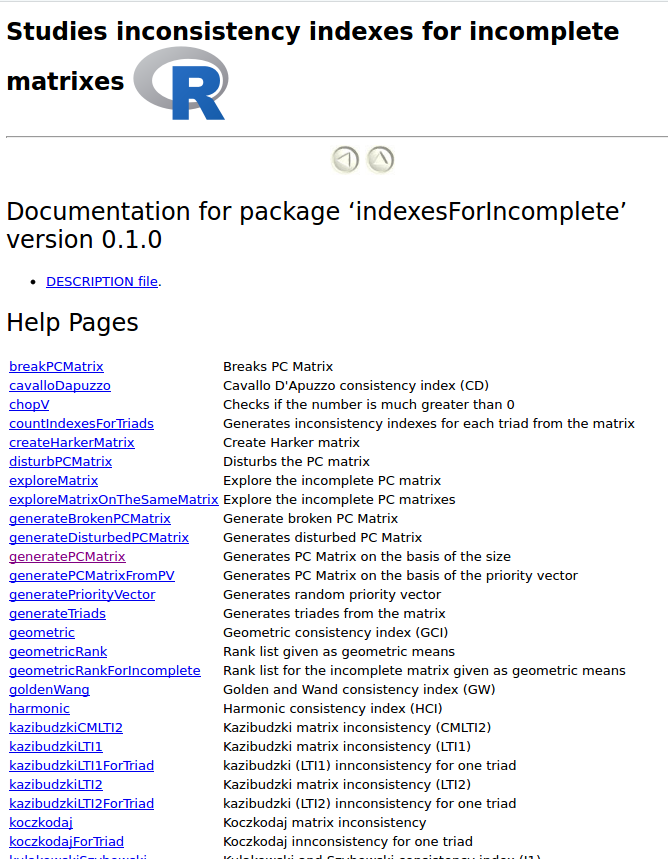
\includegraphics[scale=0.58]{images/kod31.png}}
\caption{The portion of the documentation: general view}
\end{figure}

\begin{figure}[h]
\centerline{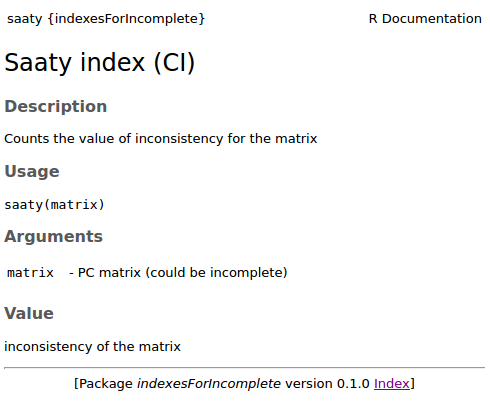
\includegraphics[scale=2.4]{images/kod32.png}}
\caption{The portion of the documentation: function \texttt{saaty}}
\end{figure}

\begin{figure}[h]
\centerline{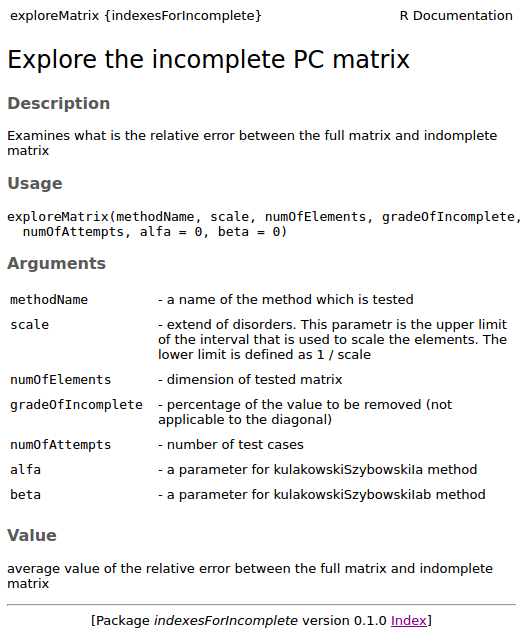
\includegraphics[scale=0.56]{images/kod33.png}}
\caption{The portion of the documentation: function \texttt{exploreMatrix}}
\end{figure}